\vspace{-3mm}

\section{Introduction} 
Federated learning (FL) enables collaborative training over decentralized data without exposing raw samples \cite{mcmahan2017communication, bonawitz2019towards}, yet the communicated updates remain vulnerable to attacks such as Deep Leakage from Gradients \cite{zhu2019deep} and Membership Inference \cite{shokri2017membership}. Differential privacy (DP) has thus become a standard safeguard in this setting \cite{zheng2021federated, naseri2020local}. Meanwhile, as foundation models such as GPT-4 \cite{achiam2023gpt}, LLaMA \cite{touvron2023llama}, PaLM2 \cite{anil2023palm}, ViT \cite{dosovitskiy2020image}, and Swin-T \cite{liu2021swin} continue to scale, fine-tuning them on resource-constrained clients quickly becomes prohibitive. Low-Rank Adaptation (LoRA) \cite{hu2022lora}, which adapts a frozen weight $W_0$ via a small low-rank update $W=W_0 +BA$, has therefore become the predominant approach for Parameter-Efficient Fine-Tuning (PEFT) in FL with foundation models, incurring minimal performance degradation compared to full fine-tuning.



However, applying LoRA in private FL is non-trivial. Its multiplicative structure induces an \emph{aggregation error} across clients, which is further amplified into a \emph{quadratic noise term} under DP-SGD, and we defer the detailed mechanism to Section \ref{sec:back}. \emph{FedLoRA} \cite{zhang2024towards}, which is the most direct adaptation of LoRA to FL, suffers from both effects and degrades sharply under tight privacy budgets and non-IID partitions. Several remedies have since been proposed to alleviate those issues. \emph{FFA-LoRA} \cite{sun2024improving} freezes $A$ and trains only $B$, \emph{RoLoRA} \cite{chen2025robust} alternates updates between $A$ and $B$ across rounds, and \emph{FedSVD} \cite{lee2025fedsvd} also trains only $B$ while applying a server-side Singular Value Decomposition (SVD). Yet all of them adopt structurally simple update strategies that impose the \emph{same mode on every layer} and follow \emph{temporally static patterns}, which overlook both the structural asymmetry between $A$ and $B$, and the round-wise variation of their relative importance. This motivates an adaptive framework in which the active LoRA component is selected per layer and per round, as depicted in Figure \ref{fig:AS-LoRA}. 


% \vspace{-0pt}
% \begin{figure}[h]
%     \centering
%     \includegraphics[width=1.0\linewidth]{./figures/1_intro/compare_huristic_v3.png}
%     \caption{Test accuracy across communication rounds under a non-private IID federated learning setting with 6 clients using the AdamW optimizer.}
%     \label{fig:compare_method}
% \end{figure}
% \vspace{-0pt}




\begin{figure}[t]
    \centering
    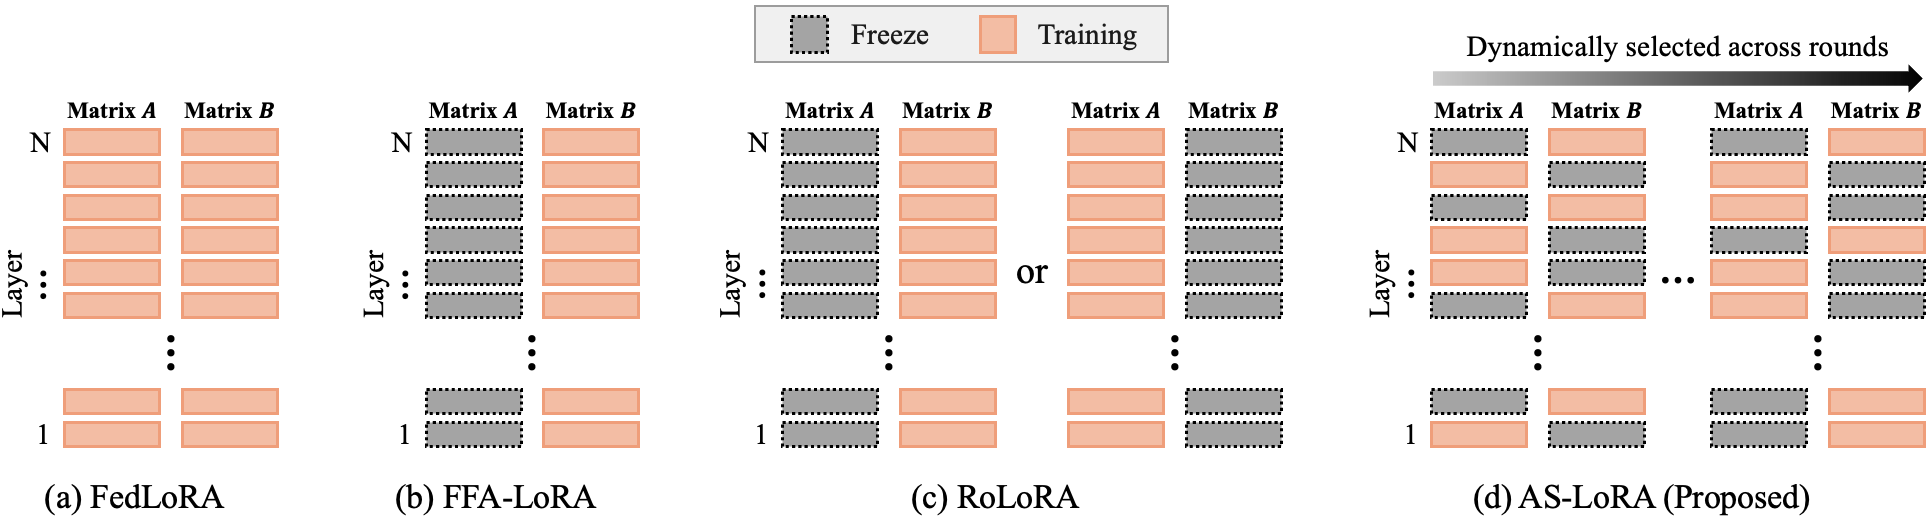
\includegraphics[width=1.0\textwidth]{./figures/1_intro/AS-LoRA_v3.png}
    \caption{Comparison of update patterns in FedLoRA, FFA-LoRA, RoLoRA, and the proposed Adaptive Selection LoRA (AS-LoRA).}
    \label{fig:AS-LoRA}
    \vspace{-20pt}
\end{figure}



\begin{wraptable}{r}{0.46\linewidth}
\centering
\vspace{-13pt}
\scriptsize
\setlength{\tabcolsep}{5.5pt}
\renewcommand{\arraystretch}{1.15}
\caption{Performance comparison of fixed alternating LoRA optimization schedules on 3 GLUE tasks. Best results are shown in \textbf{bold} and second-best results are \underline{underlined}.}
\label{tab:fixed_schedule}
\begin{tabular}{lcccc}
\toprule
\textbf{Schedule} & \textbf{MNLI (m)} & \textbf{MNLI (mm)} & \textbf{SST-2} & \textbf{QQP} \\
\midrule
\texttt{BA} \cite{chen2025robust} & \textbf{81.17} & \underline{81.96} & 92.09 & \underline{84.45} \\
\texttt{BAA} & 80.26 & 81.20 & \textbf{92.89} & 84.21 \\
\texttt{BBA} & \underline{81.10} & \textbf{81.98} & 92.30 & \underline{84.45} \\
\texttt{BBAA} & 80.78 & 81.55 & \underline{92.66} & \textbf{84.49} \\
\bottomrule
\end{tabular}
\end{wraptable}




In fact, prior work~\cite{hayou2024lora+} shows that the two low-rank matrices contribute asymmetrically to the optimization process across training stages, owing to their different initialization schemes and structural characteristics. To examine whether this asymmetry can be handled by simple fixed schedules, we conduct preliminary experiments that compare several alternating patterns including \texttt{BA}, \texttt{BBA}, and \texttt{BAA}, as shown in Table~\ref{tab:fixed_schedule}. No single schedule attains the best performance across all tasks, which indicates that fixed and heuristic alternating schedules are inherently suboptimal, and that the choice of which low-rank component to optimize should instead be made adaptively according to current training dynamics. Consistent with this observation, the active LoRA component selected by our proposed AS-LoRA varies dynamically across both layers and communication rounds throughout training, as illustrated in Figure~\ref{fig:selected}, which presents a representative trajectory whose full details are deferred to Appendix~\ref{sec:Appendix D}.

Building on those observations, we propose AS-LoRA (Adaptive Selection LoRA), and the main contributions of this paper are summarized as follows.

\begin{wrapfigure}{r}{0.45\linewidth}
\centering
\vspace{-23pt}
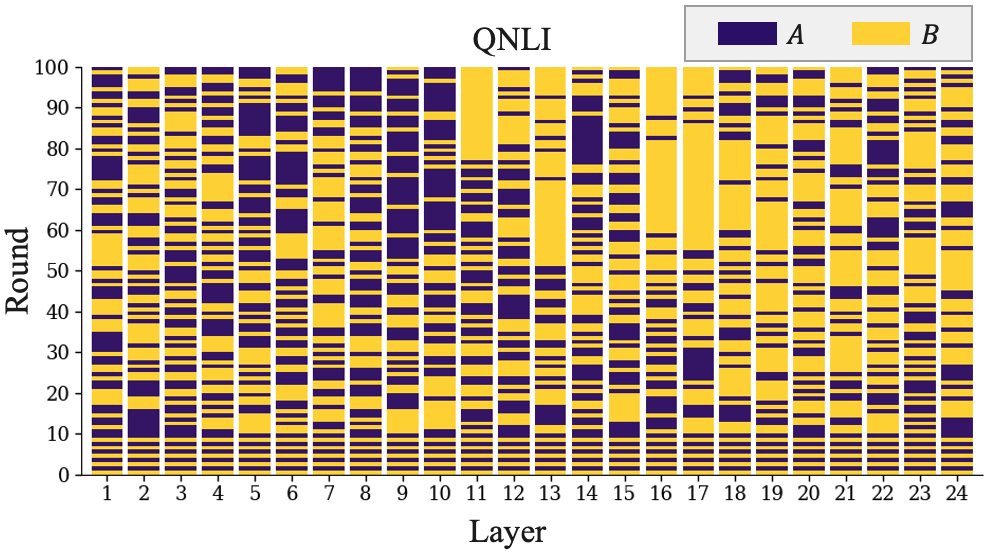
\includegraphics[width=\linewidth]{./figures/8_appendix/mode_qnli.png}
\caption{Selection of LoRA components with AS-LoRA (ours) on QNLI across layers/rounds. Different layers favor different components, and the preferred component varies across rounds, supporting the need for adaptive selection.}
\label{fig:selected}
\vspace{-5pt}
\end{wrapfigure}
\textbf{Layer-wise adaptive LoRA optimization.}
To the best of our knowledge, this is the first work that extends alternating LoRA optimization to a adaptive selection framework. We further prove that this layer-wise freedom eliminates the irreducible reconstruction-error floor that any layer-tied schedule must incur.\\
\textbf{Round-wise adaptive mode selection.}
We introduce a temporally adaptive mechanism that updates the selected LoRA component across communication rounds based on EMA-smoothed historical scores, which allows the model to adjust its optimization strategy as training progresses.\\
\textbf{Curvature-aware scoring function.}
We design a scoring function derived from a second-order approximation of the loss, which captures curvature-aware component importance. We prove that this score-driven selection accelerates convergence with a quantifiable gain over fixed schedules and implicitly biases solutions toward flatter minima, which we further verify empirically through loss-landscape and sharpness analyses. To handle the channel-wise gradient outliers that are characteristic of LoRA~\cite{jung2025gralora}, we further apply a Gaussian random projection \cite{johnson1984extensions}, which yields more reliable score estimates. \\
\textbf{Privacy at no extra cost.}
We prove that the data-dependent component selection of AS-LoRA incurs no additional privacy cost beyond standard DP-SGD, which follows from the post-processing invariance of DP.




